% ==============================================================
% Baixado de https://github.com/Swepz/latex-templates/tree/main
% Adaptado por Rianne P. Lopes (https://github.com/rianneplopes)
% ==============================================================

\documentclass[conference]{IEEEtran}
% Include all packages from file.
% Report template for Mälardalen University
% Original template can be found: 
% https://www.overleaf.com/latex/templates/ieee-bare-demo-template-for-conferences/ypypvwjmvtdf
% Template file structure organised by: Emil Persson
% The following packages should follow the IEEE conference guidelines.

% Language package 
\usepackage[utf8]{inputenc}
\usepackage[T1]{fontenc}
\usepackage[english, portuguese]{babel}


% Graphics
\usepackage{graphicx, float, subfigure, blindtext}

\newcommand\IEEEhyperrefsetup{
bookmarks=true,bookmarksnumbered=true,%
colorlinks=true,linkcolor={black},citecolor={black},urlcolor={black}%
}

% Preferred hyperref setup, Michael Shell
\usepackage[\IEEEhyperrefsetup, pdftex]{hyperref}

% Maths
\usepackage{mathtools}
\newcommand{\cmd}[1]{\texttt{#1}}

% These packages must be at the end
\usepackage[nolist,nohyperlinks]{acronym}
\usepackage{cleveref}
\graphicspath{{images/}}

% Remove section first paragraph indent
\usepackage{titlesec}
\titlespacing*{\section}{0pt}{*1}{*1}
\titlespacing*{\subsection}{0pt}{*1}{*1}
\renewcommand{\thesubsubsection}{\arabic{subsubsection}}
\titleformat{\subsubsection}[runin]{\itshape}{\thesubsubsection)}{1em}{}[:]
\titlespacing*{\subsubsection}{\parindent}{0pt}{*1}

% Include authors 
\author{\IEEEauthorblockN{ %
Rianne Passos Lopes,
Silionamã Pereira Dantas,
Maria Cecília Feitoza Gomes
}
\IEEEauthorblockA{
CHS0007 - Tópicos Especiais em Sistemática, Uso e Conservação da Biodiversidade III 2026.1 (Bioinformática) \\
Programa de Pós-Graduação em Sistemática, Uso e Conservação da Biodiversidade - Universidade Federal do Ceará \\
}}

% ACRONYMS: \acrodef{acronym}[short name]{full name}
% \acrodef{svm}[SVM]{Support Vector Machine}

% The report title.
\title{Diversidade de peixes em eDNA metabarcoding: abordagem comparativa entre ambientes natural e artificial (recife de coral vs. aquário)}
% Document begins here
\begin{document}
% Create the title.
\maketitle
% Example sections, name them
% according to specific needs.
\section{Introdução}
\label{section:intro}

Tecnologias inovadoras baseadas em DNA, que buscam a caracterização da diversidade biológica em larga escala, têm sido amplamente difundidas. Uma das técnicas mais utilizadas é a análise de amostras de DNA ambiental (eDNA) \cite{Ficetola.etal2008}. As amostras de eDNA são amplificadas utilizando iniciadores (primers) para regiões de interesse previamente definidas, e posteriormente submetida ao sequenciamento de alta geração de dados (High Throughput Sequencing – HTS). Esse processo garante a identificação taxonômica de um pool de espécies a partir de uma pequena amostra, sem a necessidade de manuseio e captura dos organismos de interesse, metodologia conhecida como eDNA metabarcoding \cite{Cristescu2014,Deiner.etal2017,Fahner.etal2016}.

Os primeiros estudos para detecção de vertebrados por eDNA foram realizados por Ficetola et al., 2008, que observaram a presença de \textit{Lithobates catesbeianus} (rã-touro-americana) em ambientes naturais e controlados. Para peixes, vários estudos mostraram eficiência de detecção nos diversos ecossistemas, como lagoas, rios, riachos e em regiões marítimas \cite{Takahara.etal2013,Sigsgaard.etal2015,Minamoto.etal2012,Thomsen.etal2012,Kelly.etal2014}. Nos ambientes aquáticos, o material genético detectado é originário de diversas fontes como tecidos deteriorados ou células da pele e estão depositados na camada superficial da água. 

Estudos com eDNA metabarcoding são ferramentas poderosas que minimizam o contato com o objeto de estudo e contribuem significativamente para o monitoramento da biodiversidade, gerando conhecimento no intuito de diminuir os impactos sobre o meio ambiente. A metodologia de eDNA metabarcoding vem sendo aplicada em projetos de monitoramentos ambiental, no intuito de avaliar a eficiência de estratégias de manejo, bem como em estudos sobre conservação da biodiversidade, atribuindo resultados rápidos e confiáveis para um conjunto de decisões regulatórias e de conservação \cite{Oliveira.etal2023}.

Porém, para análise de composição de comunidades e avaliação de biodiversidade com a metodologia de DNA metabarcoding são necessários protocolos eficientes em cada uma de suas etapas. Uma das etapas mais críticas  desses estudos é a seleção do marcador molecular e dos iniciadores, que determina a capacidade de detecção da comunidade alvo. Para o monitoramento de comunidades ictiológicas, o gene mitocondrial 12S rRNA é amplamente consolidado como marcador padrão para DNA ambiental.

Os primers MiFish \cite{Miya.etal2015a} são um conjunto de iniciadores universais projetados especificamente para amplificar um fragmento curto de aproximadamente 170 pares de base do gene 12S rRNA. Esses primers demonstraram uma alta capacidade de discriminar táxons de peixes, tanto teleósteos quanto elasmobrânquios. Para a validação do MiFish, os autores originais realizaram análises que contrastaram ambientes naturais com ambientes controlados cuja composição da biodiversidade era previamente conhecida, a fim de testar e aferir a sensibilidade dos iniciadores.

Diante disso, este projeto utilizou uma fração dos dados de sequenciamento depositados no DNA Databank of Japan (DDBJ) pelo bioprojeto original do MiFish. O objetivo geral de nosso projeto foi avaliar e comparar a estrutura, riqueza e composição taxonômica da comunidade de peixes entre o ecossistema natural do Recife de Bise e o ambiente controlado do Aquário Churaumi utilizando metabarcoding de eDNA. Para alcançar este propósito, os objetivos específicos delineados foram a implementação de um pipeline reprodutível no ambiente QIIME 2 para a resolução de Variantes de Sequência de Amplicons (ASVs), a comparação dos índices de diversidade alfa (riqueza observada) e beta (similaridade por distância de Jaccard) entre os dois ambientes, e, por fim, a avaliação comparativa do perfil e composição das famílias de peixes detectadas em cada ambiente.
\section{Material e métodos}
\label{section:method}

O pipeline foi executado em um ambiente contêiner baseado em Ubuntu 24.04. A automação e o gerenciamento das ferramentas foram estruturados via Miniforge3, criando-se o ambiente virtual \cmd{qiime2\_amplicon}. Este ambiente integrou nativamente o QIIME 2 (v. 2024.10) e as dependências em Python 3.10 utilizadas para as análises estatísticas e gráficos (JupyterLab, pandas, seaborn e matplotlib), além dos utilitários de terminal cutadapt, pigz e sra-tools.

Os dados de sequenciamento paired-end foram obtidos a partir do repositório público DNA Databank of Japan, sob o esforço amostral de n = 8 corridas de sequenciamento (IDs: \cmd{DRR030421}-\cmd{DRR030428}). O desenho experimental consistiu em quatro réplicas biológicas para o ambiente artificial controlado (Aquário Churaumi) e quatro réplicas para o ambiente marinho natural (Recife de Corais de Bise, Okinawa, Japão). O download automatizado dos arquivos originais em formato \cmd{.sra} foi realizado via protocolo HTTP, seguido da extração das leituras brutas demultiplexadas em arquivos FASTQ pareados utilizando a ferramenta \cmd{fasterq-dump} (sra-tools). Os arquivos foram compactados com o algoritmo \cmd{pigz} para otimização de armazenamento.

As análises de bioinformática foram centralizadas no ambiente QIIME 2. Inicialmente, um arquivo de manifesto contendo os caminhos absolutos das leituras foi estruturado para importação das sequências brutas pelo formato \cmd{PairedEndFastqManifestPhred33V2}, gerando o artefato base de dados pareados com qualidade Phred-33. A remoção estrita dos primers foi executada com o comando \cmd{qiime cutadapt trim-paired}, que buscou as sequências do marcador universal MiFish na região do gene mitocondrial 12S rRNA (Forward MiFish-U-F: \cmd{5'-GTCGGTAAAACTCGTGCCAGC-3'}) e Reverse (MiFish-U-R: \cmd{5'-CATAGTGGGGTATCTAATCCCAGTTTG-3'}), com correspondência de caracteres curinga. O perfil de qualidade das leituras antes e após a remoção dos primers foi inspecionado visualmente por meio do comando \cmd{qiime demux summarize}.

As leituras limpas foram submetidas ao algoritmo DADA2 via comando \cmd{qiime dada2 denoise-paired} para correção de erros de sequenciamento, filtragem por qualidade, fusão de fitas (paired-end merging) e remoção de quimeras pelo método consensus. Após inspeção da qualidade das corridas, os parâmetros de truncamento foram fixados em 120 pb para as leituras Forward e 115 pb para as Reverse, sem cortes à esquerda (\cmd{trim-left = 0}), garantindo uma zona de sobreposição (overlap) segura de aproximadamente 65 pb para o acoplamento. As Variantes de Sequência de Amplicons (ASVs) resultantes foram tabuladas e classificadas taxonomicamente utilizando um classificador probabilístico Naive Bayes treinado pelo comando \cmd{qiime feature-classifier fit-classifier-naive-bayes}. O treinamento, direcionado para a região do gene 12S amplificada pelos iniciadores, teve como base a biblioteca de referência curada e especializada Mitohelper \cite{Lim.Thompson2021}.

A matriz de abundâncias foi padronizada por rarefação em uma profundidade fixa de 45.000 reads por amostra, valor determinado pela estabilização das curvas e formação do platô inspecionados pelo comando \cmd{qiime diversity alpha-rarefaction}. O valor de 45.000 normalizou o esforço amostral, garantindo que nenhuma das oito amostras fosse excluída das análises de diversidade e mitigou as disparidades na profundidade de sequenciamento. A diversidade alfa (riqueza de ASVs e índice de Shannon) foi calculada pelo comando \cmd{qiime diversity core-metrics}. A diferença entre as medianas dos dois ambientes foi avaliada pelo teste não-paramétrico de Kruskal-Wallis. A diferença na composição de comunidades (diversidade beta) foi estimada através das matrizes de distância de Jaccard, ordenadas por Análise de Coordenadas Principais (PCoA). A diferença entre os ambientes foi testada por Análise de Variância Molecular Permutacional (PERMANOVA) com 999 permutações.

\section{Resultados e Discussão}
\label{section:results-n-discussion}

As curvas de rarefação demonstraram que as amostras sequenciadas em ambos os ambientes atingiram o platô de saturação antes da profundidade crítica fixada, indicando sucesso na amostragem da comunidade ictiológica. A linha de corte, definida em 45.000 reads, garantiu alta cobertura biológica de ambos os cenários, preservando o equilíbrio do desenho experimental e mitigando vieses de disparidade de sequenciamento (Figura~\ref{fig:curva_rarefacao_asvs}).

\begin{figure}[H]
    \centering
    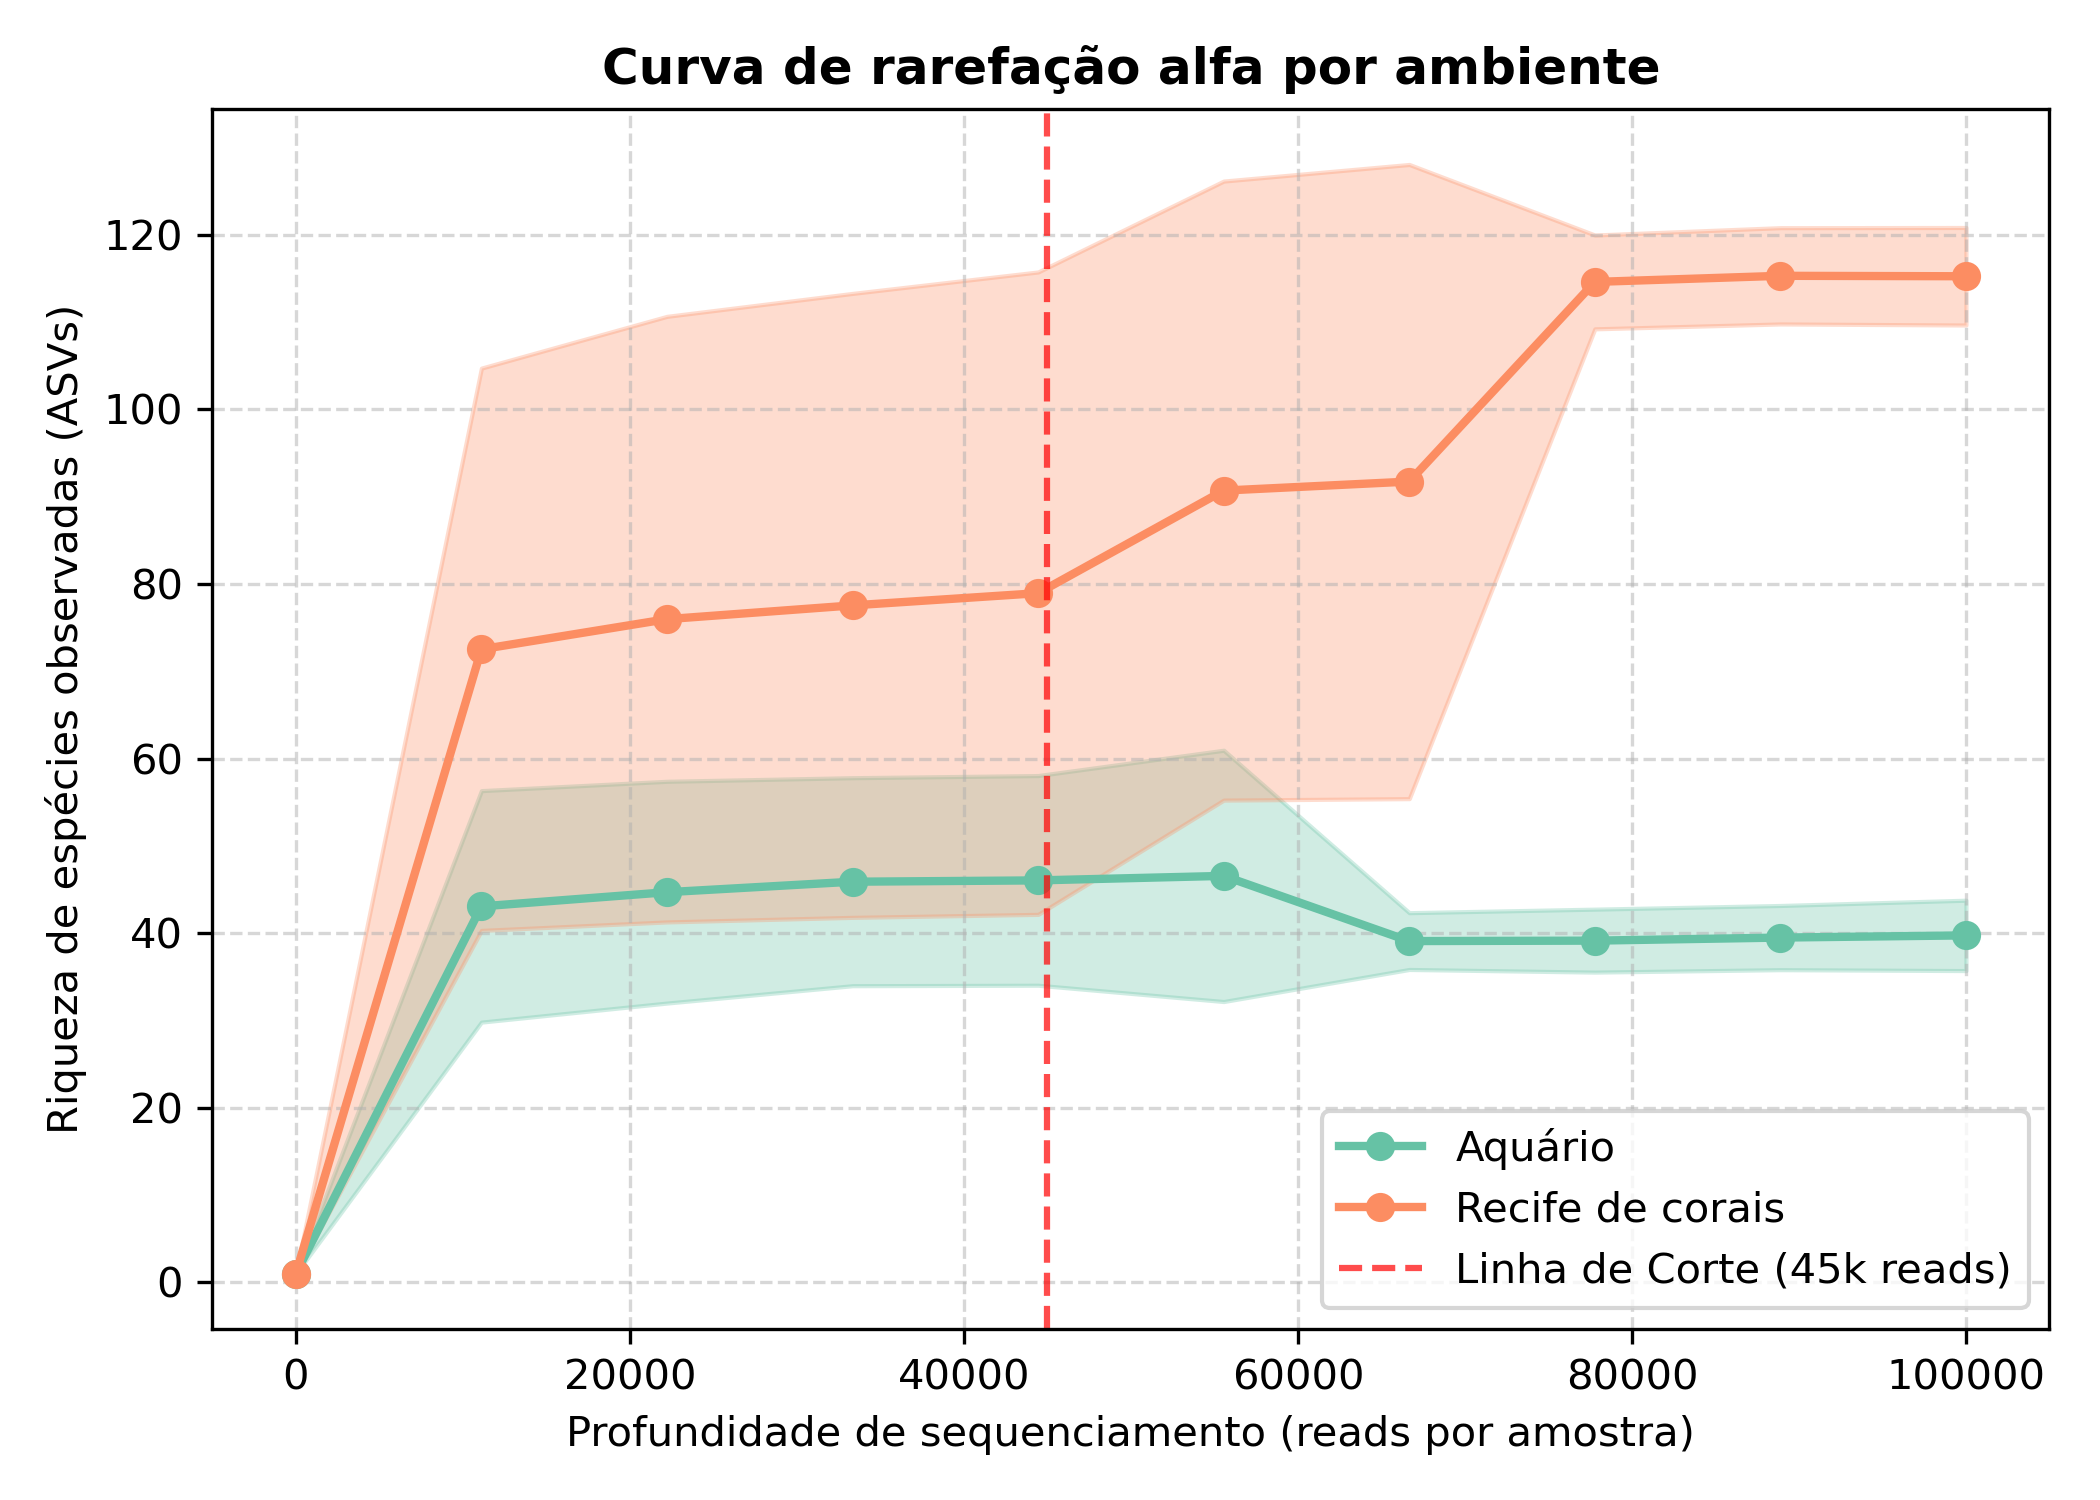
\includegraphics[width=0.7\columnwidth]{curva_rarefacao_asvs}
    \caption{Curva de rarefação das amostras após o processamento das sequências. A linha vertical representa o ponto de amostragem adotado (45.000 reads) para normalização.}
    \label{fig:curva_rarefacao_asvs}
\end{figure}

Em relação à diversidade alfa, o ambiente do Recife de Bise apresentou uma riqueza mediana de Variantes de Sequência de Amplicons (ASVs) de aproximadamente 80 ASVs, enquanto o ambiente artificial do Aquário Churaumi apresentou uma mediana de aproximadamente 40 ASVs (Figura~\ref{fig:boxplot_riqueza}). As medianas não diferiram entre os ambientes para as amostras analisadas ($H = 2,13$; $p = 0,14$). Os dados do aquário mostraram-se mais homogêneos devido ao ambiente fechado e controlado, enquanto o recife está sujeito a variações por múltiplos fatores ecológicos e físicos observados em ambientes naturais.

\begin{figure}[H]
    \centering
    
\includegraphics[width=0.8\columnwidth]{boxplot_riqueza}
    \caption{Variabilidade da diversidade alfa para a comunidade ictiológica estimada via metabarcoding de eDNA, dada pela riqueza de Variantes de Sequência de Amplicons (ASVs) observadas.}
    \label{fig:boxplot_riqueza}
\end{figure}

Por outro lado, a estrutura de diversidade beta revelou uma separação espacial entre as comunidades ($\text{Pseudo-F} = 1,73$; $p = 0,031$; 999 permutações). A Análise de Coordenadas Principais (PCoA) evidenciou um agrupamento coeso e restrito para as amostras do Recife de Coral, indicando alta homogeneidade e compartilhamento de táxons no ecossistema natural aberto (Figura~\ref{fig:pcoa_jaccard}). Inversamente, o Aquário Churaumi exibiu uma expressiva variação interna ao longo do eixo vertical (PC2), fragmentando-se em dois subgrupos. Essa segregação reflete o isolamento biológico entre os tanques artificiais, onde cada recinto confina composições diferentes de espécies. Esse padrão demonstra que, embora o número absoluto de espécies (alfa) não difira estritamente, a composição das espécies presentes é consideravelmente distinta, com alta turnover taxonômico entre os ambientes.

\begin{figure}[H]
    \centering
    
\includegraphics[width=0.9\columnwidth]{pcoa_jaccard}
    \caption{Ordenação por Análise de Coordenadas Principais (PCoA) baseada na matriz de distância de Jaccard para a composição de peixes. Os eixos representam a porcentagem de variação total explicada pelos dados.}
    \label{fig:pcoa_jaccard}
\end{figure}

O perfil taxonômico por corrida de sequenciamento (Figura~\ref{fig:barplot_taxonomia_n8}) corroborou o padrão de diversidade beta, exibindo consistência entre as réplicas do Recife e forte heterogeneidade entre os tanques do Aquário. No nível de Família, evidenciou-se uma inversão quase total de dominância taxonômica entre os dois ecossistemas (Figura~\ref{fig:barplot_taxonomia}). No ambiente controlado do Aquário, as análises mostraram dominância das famílias Monodactylidae e Gempylidae, refletindo as espécies selecionadas para estocagem biológica nos tanques de exibição. Em contrapartida, essas famílias mostraram-se ausentes no ecossistema natural do Recife de Bise, onde a comunidade foi caracterizada pela dominância de peixes recifais típicos das famílias Belonidae, Blenniidae e Pomacentridae. 

\begin{figure}[H]
    \centering
    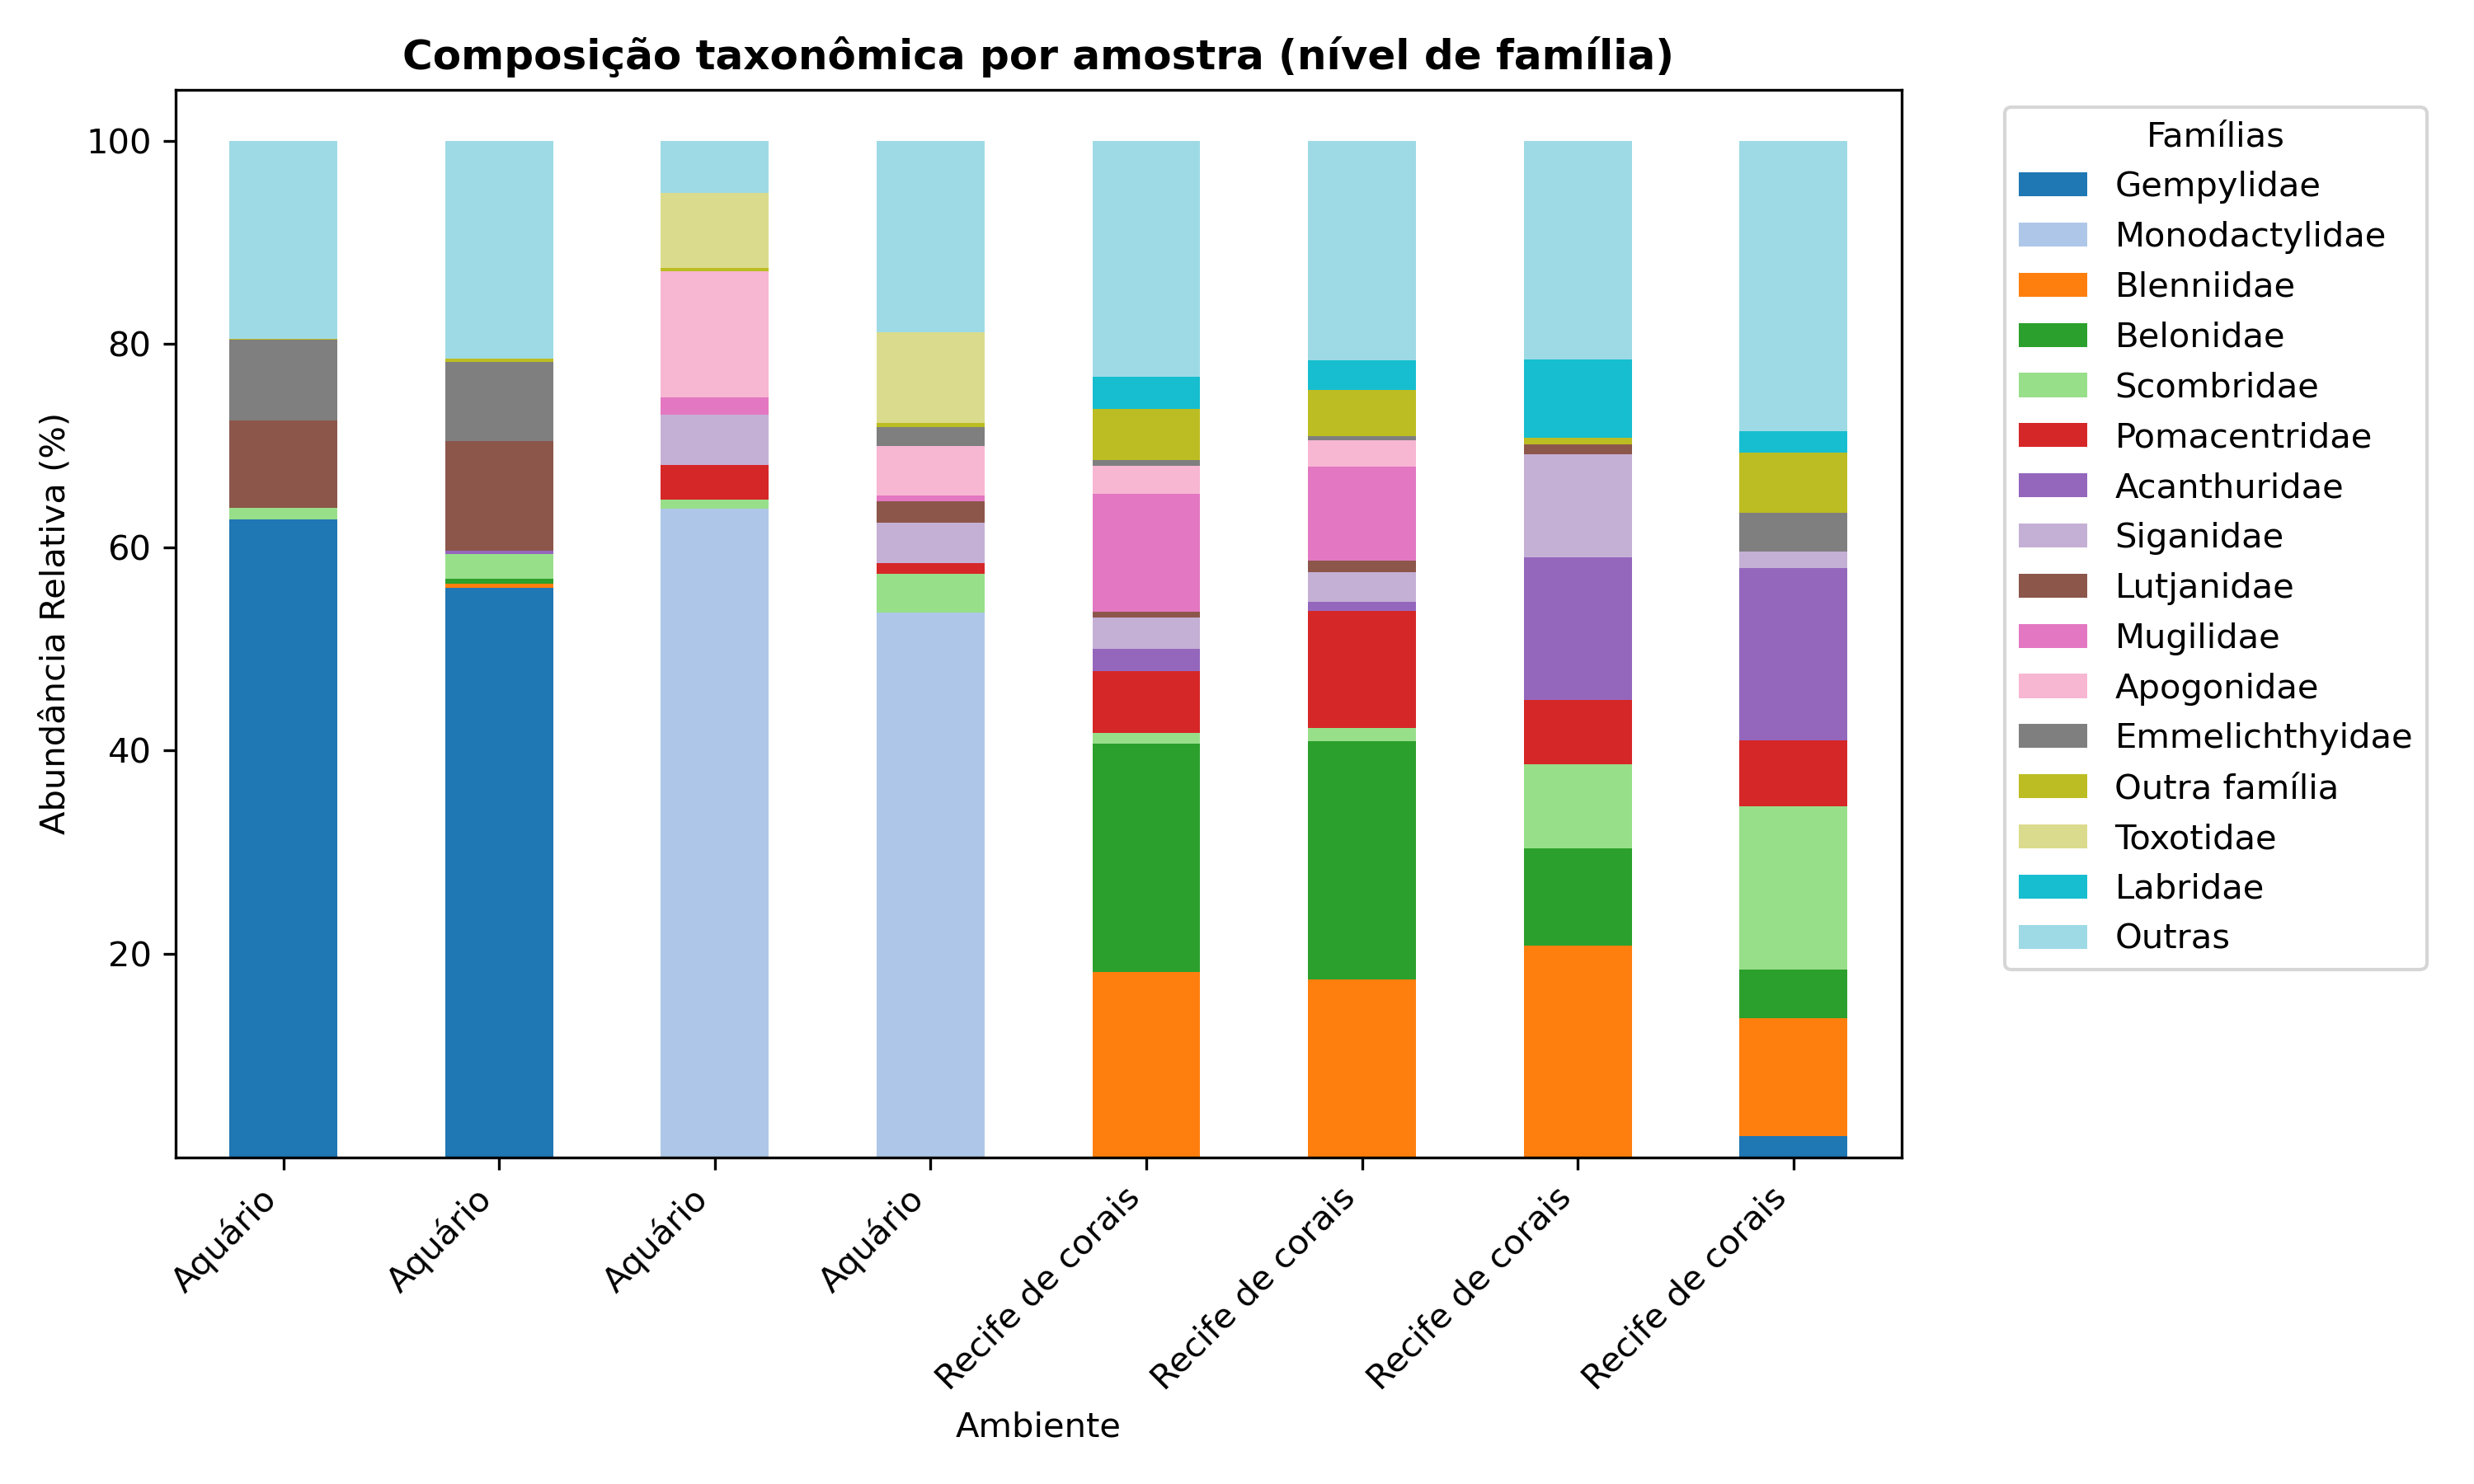
\includegraphics[width=0.8\columnwidth]{barplot_taxonomia_n8}
    \caption{Composição taxonômica relativa e perfil de distribuição de leituras da comunidade de peixes por corrida de sequenciamento ($n = 8$). As abundâncias estão agregadas em nível de Família para as 4 réplicas do Aquário Churaumi e as 4 réplicas do Recife de Bise. Famílias abaixo das 15 mais abundantes foram agrupadas na categoria "Outros".}
    \label{fig:barplot_taxonomia_n8}
\end{figure}

Diante dos resultados acima apresentados, podemos concluir que as composições entre os dois ambientes dos quais foram extraídas as amostras (Aquário e Recife de Coral) é distinta em termos de riqueza de espécies. O ambiente de Recife de Coral possui maior riqueza, com aproximadamente o dobro de espécies em relação ao ambiente artificial. Há uma inversão de dominância taxonômica entre os ambientes: as famílias dominantes no ambiente de Aquário (Monodactylidae e Gempylidae) são irrelevantes no ambiente de Recifes de corais (Belonidae, Blenniidae e Pomacentridae).

\begin{figure}[H]
    \centering
    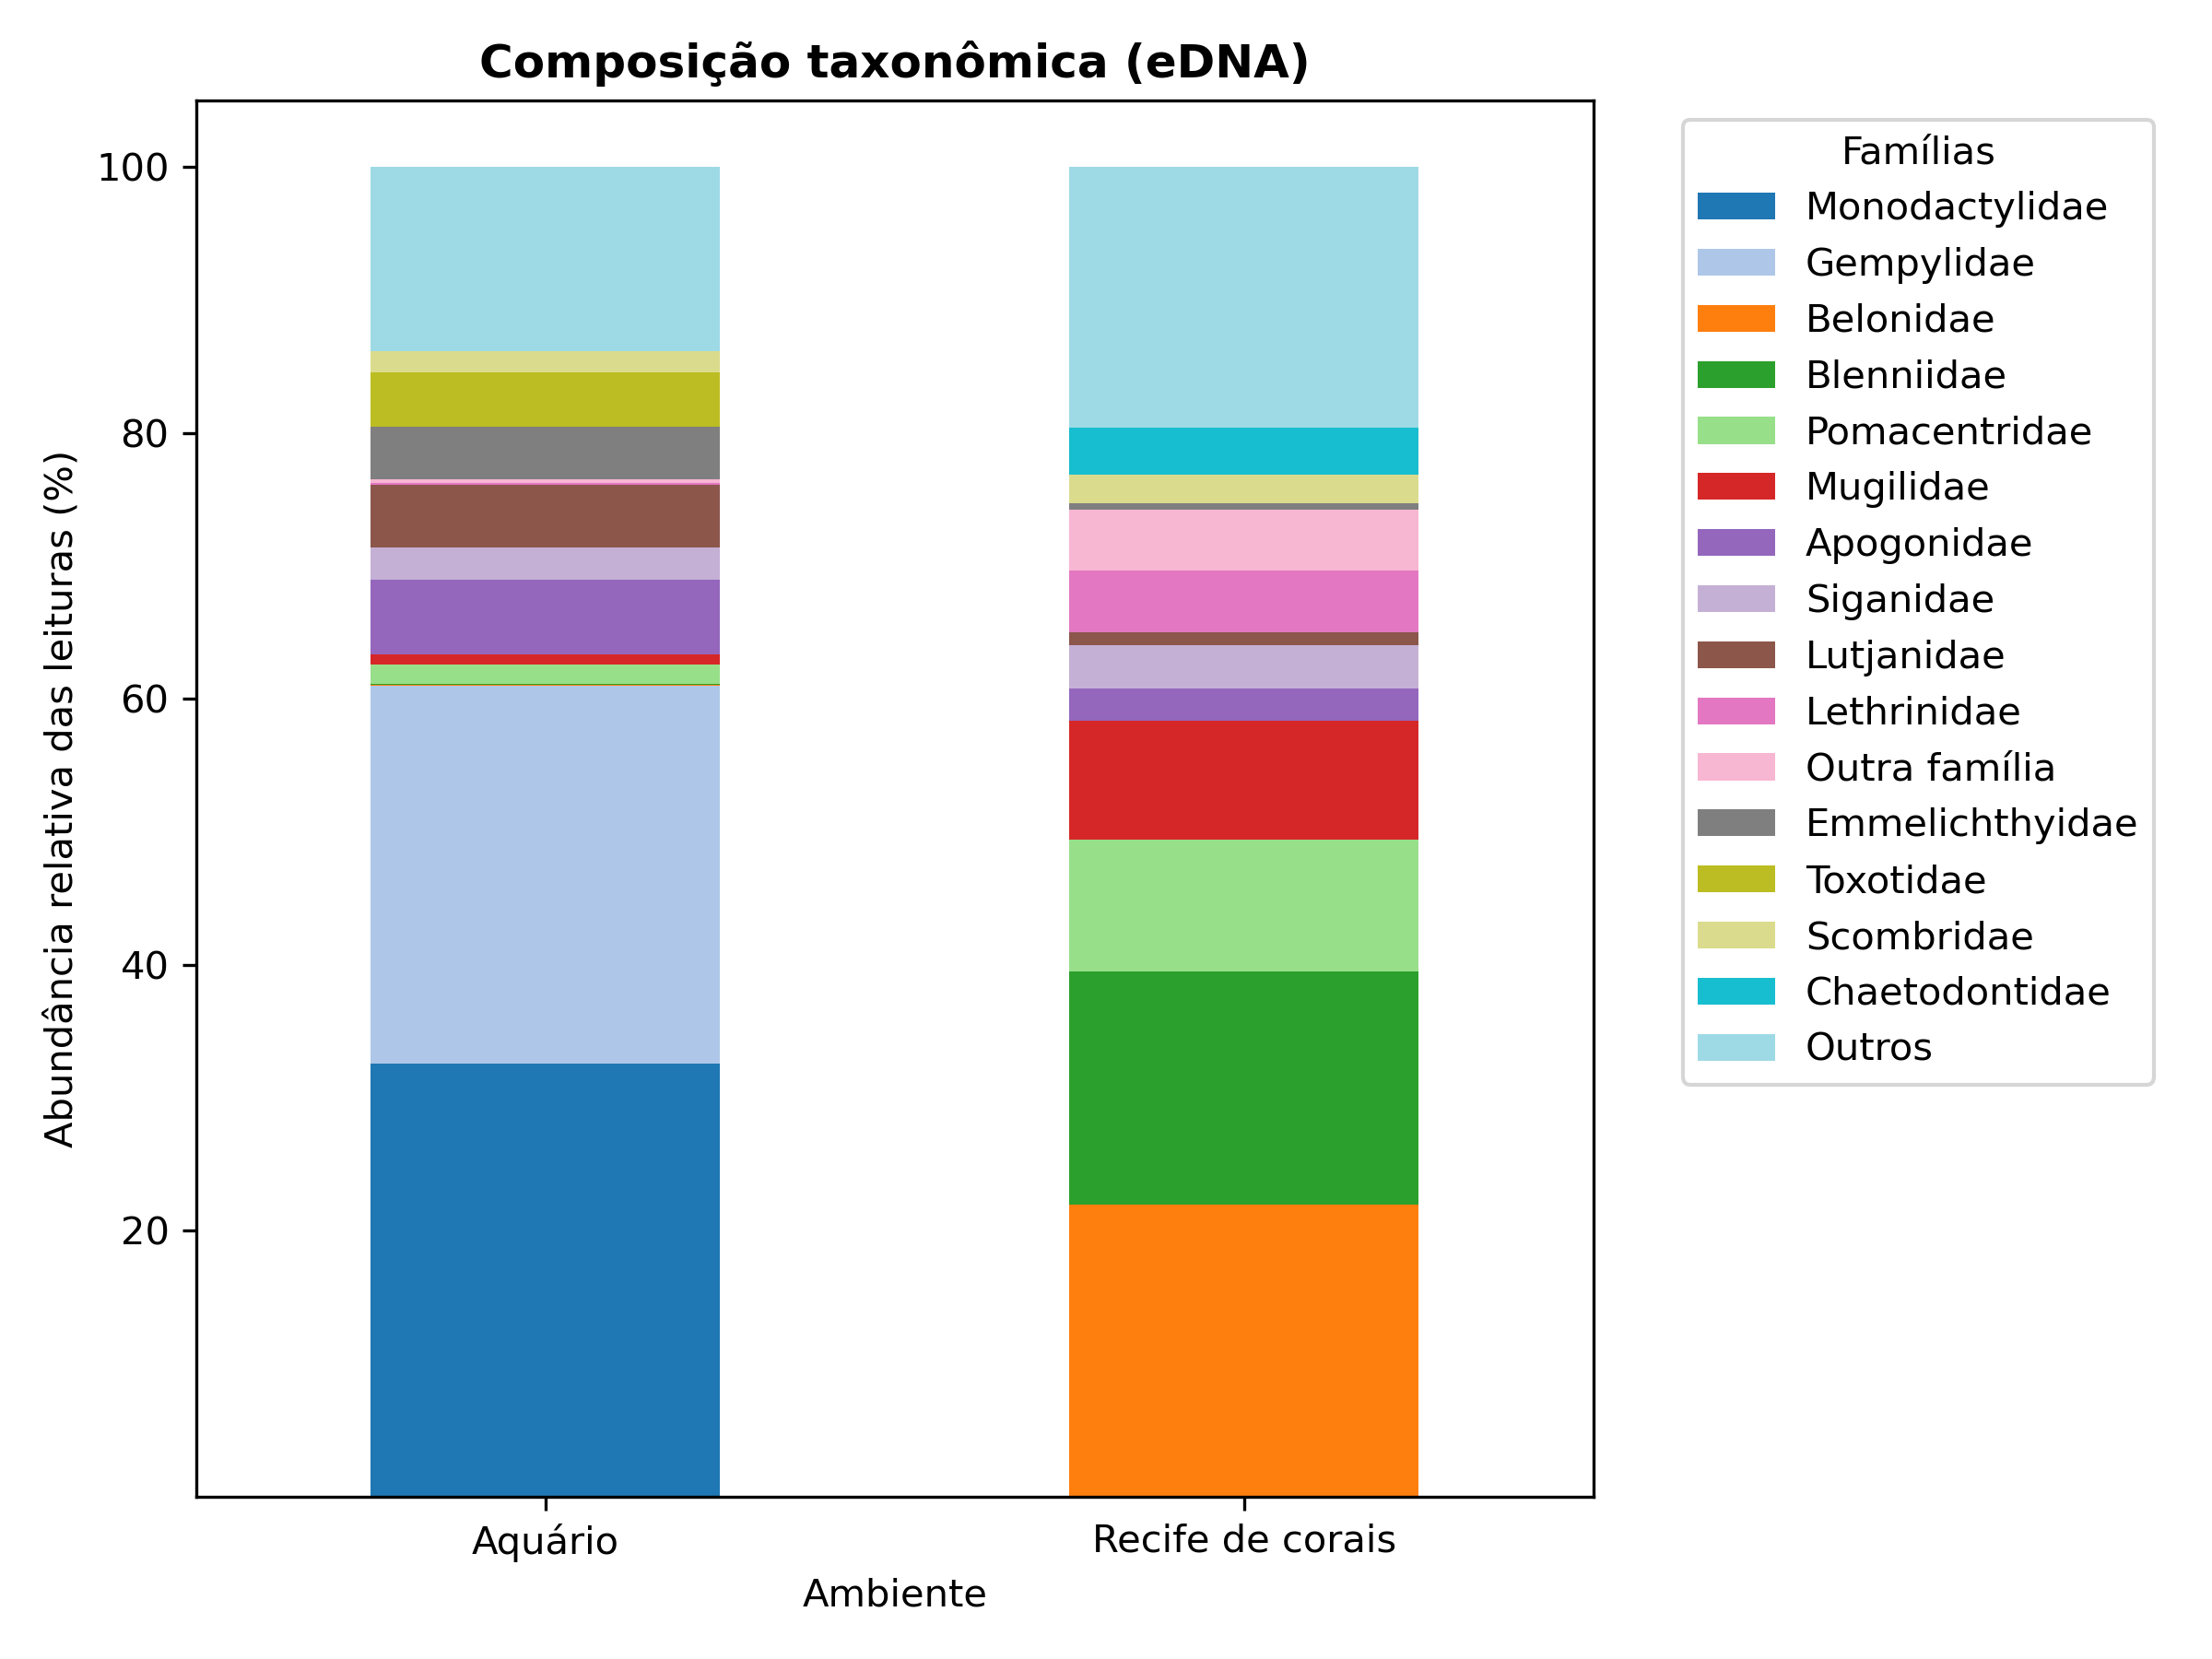
\includegraphics[width=0.8\columnwidth]{barplot_taxonomia}
    \caption{Comparação do perfil taxonômico médio da ictiofauna agrupado por tipo de ambiente. As barras empilhadas representam a abundância relativa agregada em nível de Família.}
    \label{fig:barplot_taxonomia}
\end{figure}

Essa divergência taxonômica evidencia a sensibilidade do marcador MiFish e a adequação do pipeline no QIIME 2. O método foi capaz de discriminar com precisão a assinatura molecular de uma comunidade artificial e controlada daquela presente em um ecossistema marinho aberto, capturando a substituição quase total das espécies (turnover) entre os ambientes.
% Select the IEEEtran style
\bibliographystyle{IEEEtran}
% Include bibliography file
\bibliography{IEEEabrv,refs}
\end{document}